\subsection{Fragebogen} \label{fragebogen-4}

\todo[inline]{Verantwortlich: Boris\\
- RfP}


F{\"u}r dieses Prototyp wurden zwei Arten von Frageb{\"o}gen benutzt. 
Der erste Typ ist sehr {\"a}hnlich mit dem von der zweite Prototyp. Es enth{\"a}lt in dem informativen Teil einen Text, wo es beschrieben wird, wie der Fragebogen ausgef{\"u}llt werden soll. Der andere Teil besteht aus vier Dropdown-Boxen von dreizehn Optionen, die zw{\"o}lf verschiedene Emotionen und einen als null oder neutral geltenden Zustand enthalten. Jede Dropdown-Box entspricht ein Viertelzeit der Szenario. Es soll zwischen die Optionen jeder Dropdown-Box gew{\"a}hlt werden, welche Emotion es am st{\"a}rksten empfindet wird, je nachdem, wann man es f{\"u}hlte, d.h. ob es das erste, zweite, dritte oder letzte Quartal der Zeit des Videos war, um die Emotion zu bew{\"a}ltigen. Unten gibt es ein Button wo man dr{\"u}cken kann, wenn man fertig ist. Allerdings hat man auch die M{\"o}glichkeit seine Wahl zu {\"a}ndern, auch wenn man sich schon im n{\"a}chsten Schritt befindet, indem man in diesem n{\"a}chsten Schritt auf den Zur{\"u}ck-Button dr{\"u}ckt und die gew{\"u}nschten {\"a}nderungen vornimmt. Hierf{\"u}r wird ein Widget Blueprint erstellt, die vier Dropdown-Boxen mit dem gew{\"u}nschten Anzahl an Optionen hinzugef{\"u}gt und die Labels von der unterschiedlichen Optionen der Dropdown-Boxen definiert. Ein Button ``next'' wird auch erstellt um zum n{\"a}chsten Fragebogen zu navigieren. Es wird auch eine zwischen Speicherungsfunktion in ein anderes Skript definiert, die hier aufgerufen wird, um die {\"a}nderung auch nach das dr{\"u}cken von dem ``next'' Button zu Speichern. Dabei wird vier Variablen definiert und die Werte von der gew{\"a}hlten Optionen werden ihnen zugewiesen. \\



\begin{figure}[H] \centering
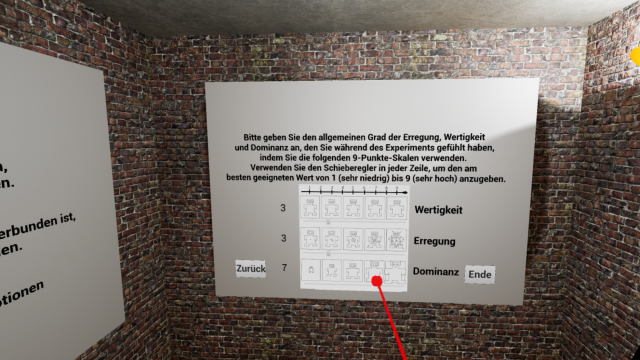
\includegraphics[width=\textwidth]{Images/Fragebogen_3.png} 
\caption{ Bild des Fragebogen-Teils, entsprechend dem circumplex-Modell. } 
\label{fig:fragenbogen4} \end{figure}



Der zweite Typ {\"a}hnelt dem ber{\"u}hmten Modell von James Russels ``circumplex'' \cite{russel_1980}. Es ist ein klassisches Modell mit einer kreisf{\"o}rmigen Struktur, die auf zwei senkrechten Diagonalen ruht. Die vertikale Achse, die die Erregung darstellt, und die horizontale Achse, die die Valenz darstellt. Das Zentrum des Kreises stellt eine neutrale Valenz und ein mittleres Erregungsniveau dar. Andere Emotionen werden auf jeder Ebene des Kreises dargestellt.  Hier wird ein weniger bekanntes Modell verwendet, das ``Self Assessment Manikin'' (SAM). Es besteht aus drei Reihen mit je f{\"u}nf Piktogrammen. Diese Piktogramme stellen den Zustand eines Gesichts nach verschiedenen Arten von Emotionen dar. So repr{\"a}sentiert der erste Bereich die Wertigkeit, der zweite die Erregung und der dritte die Dominanz. Eine Erkl{\"a}rung zu jedem dieser Begriffe ist ebenfalls neben dem Fragebogen enthalten, um die Testpersonen {\"u}ber diese W{\"o}rter aufzukl{\"a}ren.  Bei jeder Avatar und in der Mitte jeder der beiden Avatar befindet sich ein Checkbox.  So muss man f{\"u}r jede Zeile das Checkbox ausw{\"a}hlen, das ihrem emotionalen Zustand am besten entspricht. Man kann nur ein Checkbox pro Zeile markieren und man hat auch die M{\"o}glichkeit wie bei dem ersten Model seine Wahl zu {\"a}ndern. Es kann einfach mit Branch-Bedingungen realisieren werden.  Diese werden auch in eine Widget Blueprint wie f{\"u}r das erste Modell gemacht. Es gibt auch wieder die zwischen Speicherungsfunktion und das Button ``next''. Was neues hier kommt ist das Button ``back'' um wieder zum ersten Fragebogen zu navigieren. 



\begin{figure}[H] \centering
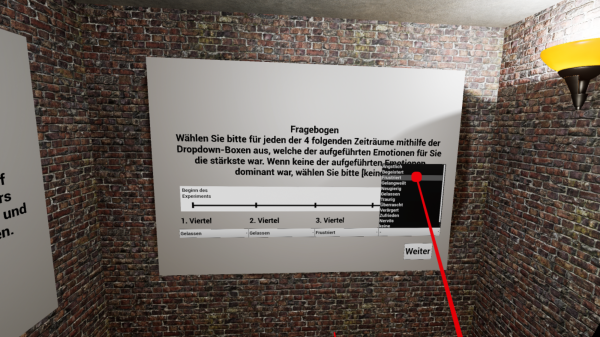
\includegraphics[width=\textwidth]{Images/Fragebogen_1.png} 
\caption{ Bild des Fragebogen-Teils, wo die dominierenden Emotionen abgefragt werden. } 
\label{fig:fragenbogen1} \end{figure}